% Created 2018-08-13 Mon 17:13
% Intended LaTeX compiler: pdflatex
\documentclass[a4paper, twocolumn]{article}
\usepackage[utf8]{inputenc}
\usepackage[T1]{fontenc}
\usepackage{graphicx}
\usepackage{grffile}
\usepackage{longtable}
\usepackage{wrapfig}
\usepackage{rotating}
\usepackage[normalem]{ulem}
\usepackage{amsmath}
\usepackage{textcomp}
\usepackage{amssymb}
\usepackage{capt-of}
\usepackage{hyperref}
\usepackage{minted}
\usepackage[margin=0.6in]{geometry}
\setlength{\columnsep}{0.4in}
\usepackage{amssymb,amsmath}
\usepackage{fancyhdr} %For headers and footers
\pagestyle{fancy} %For headers and footers
\fancyfoot[CE,CO]{}
\fancyhead[LE,LO]{}
\usepackage{lastpage} %For getting page x of y
\usepackage{float} %Allows the figures to be positioned and formatted nicely
\restylefloat{figure} %and this command
\usepackage{hyperref}
\hypersetup{urlcolor=blue}
\usepackage{titlesec}
\setcounter{secnumdepth}{4}
\usepackage{minted}
\setminted{frame=single,framesep=10pt}
\chead{}
\rhead{Section: \thesection}
\rfoot{\thepage\ of \pageref{LastPage}}
\usepackage[parfill]{parskip}
\usepackage{subfig}
\hypersetup{colorlinks=true,linkcolor=black, citecolor=black}
\usepackage[none]{hyphenat}
\usepackage{framed}
\author{NH, CN, HO, JD}
\date{\today}
\title{Domestication Draft}
\hypersetup{
 pdfauthor={NH, CN, HO, JD},
 pdftitle={Domestication Draft},
 pdfkeywords={},
 pdfsubject={},
 pdfcreator={Emacs 27.0.50 (Org mode 9.1.9)},
 pdflang={English}}
\begin{document}

\maketitle
% Redefine the plain page style
\fancypagestyle{plain}{%
  \fancyhf{}%
  \renewcommand{\headrulewidth}{0pt}% Line at the header invisible
  \rfoot{\thepage\ of \pageref{LastPage}}
  \fancyfoot[CE,CO]{}
}

% \patchcmd{\chapter}{\thispagestyle{fancy}}{\thispagestyle{fancy}}{}{}


\section{Introduction}
\label{sec:org1e43827}
<Waiting for Hugo>

\section{{\bfseries\sffamily TODO} }
\label{sec:org48c2e01}

\begin{itemize}
\item[{$\square$}] Report on standard deviations and errors, would be very interesting to highlight changes in this from prim to domesticated.
\end{itemize}

\section{Results}
\label{sec:org0b43068}

Previous research demonstrated that certain species of wheat underwent a significant (a two-thirds increase) biomass shift during domestication \cite{Waines2007}. Several more studies have confirmed the expected grain filling, volume and size change undergone during domestication \cite{Gupta2006,Piperno2004}, but have been unable to provide detailed explanation of the effects leading to the observed changes in grain morphology.

\begin{figure}[htbp]
\centering
\includegraphics[width=8cm]{/home/nathan/Dropbox/NPPC/Domestication/Figures/fig1.png}
\caption{\label{fig:org29a60ba}
Einkorn (top) and Emmer (bottom) Wheat (Primitives left, Domesticated right)}
\end{figure}

Four key species, two diploid (Einkorn) and two tetraploid (Emmer) were selected to study the effect on grain morphology across domestication and polyploidisation. Domesticated  \emph{T. monococcum} and primitive \emph{T. boeticum} were selected for being diploid; Domesticated \emph{T. dicoccum} as primitive \emph{T. dicoccoides} were chosen as representative species for tetraploids. (See Figure 1)

Key grain morphological traits were measured using micro-CT imaging, these include length, width, depth, volume, and surface area. From these traits, two additional descriptors were created LWD (Length X Width X Depth) and Surface area / Volume ratio these are used to provide insight to potential trait interactions. Of these traits, length and width have already been highlighted as having vital importance in building genetic frameworks for wheat \cite{Gegas2010}.

Traits were gathered using image analysis software \cite{Hughes2017}, major modifications were made to grain identification algorithms in order to adapt to the wide variety in the species studied.

Analysis was performed using a Welch T-test for significance and confidence intervals. Kruchke's method was used for Bayesian estimation of difference \cite{Kruschke2012} in order to quantify differences in population means. Estimation of domestication status was achieved through multiple regression (using ordinary least squares methods).

Principle Component Analysis (PCA) was used to highlight separation of species based on grain measurements, in addition to the effect of specific traits in model though reported eigenvalues/coefficient loadings.

\subsection{Einkorn}
\label{sec:orgdb48674}

\subsubsection{Grain Traits}
\label{sec:org95473f6}
No noticeable change has been observed in the length attribute between domesticated and wild einkorn (\(p=0.02\) and a predicted \(35\%\) probability of overlapping averages).

\begin{figure}[htbp]
\centering
\includegraphics[width=9cm]{/home/nathan/Dropbox/NPPC/Domestication/Figures/fig2.png}
\caption{\label{fig:orgec63b81}
Einkorn Traits}
\end{figure}

However, other traits(figure:2): length, width, depth, volume and surface area all have a significant change between wild and domesticated (\(p<0.01\)).


\subsubsection{Principle Component Analysis}
\label{sec:orgd9ffcf8}
A two component PCA reviled that no dominant trait appears to influence morphometric variation in einkorn species (figure:3).

\begin{figure}[htbp]
\centering
\includegraphics[width=9cm]{/home/nathan/Dropbox/NPPC/Domestication/Figures/fig3.png}
\caption{\label{fig:org69ae4ca}
Einkorn PCA}
\end{figure}

With the exception of grain length (-0.24), all other measurements (width, depth, volume, surface area and the interaction term LxWxD) have coefficients ranging -0.38 to -0.46 in the first principle component (76.77\% of explained variation).

\subsection{Emmer}
\label{sec:orgf51c491}

\subsubsection{Grain Traits}
\label{sec:org013bee9}
With length, Emmer displays no significant difference in grain length between wild and domesticated species (\(p=0.93\)).

\begin{figure}[htbp]
\centering
\includegraphics[width=9cm]{/home/nathan/Dropbox/NPPC/Domestication/Figures/fig4.png}
\caption{\label{fig:org6f3821f}
Emmer Traits}
\end{figure}


Additionally, surface area of grain is reported as non-significant (\(p=0.17\)). Showing that grain compactness has significantly altered to preserve this trait (Figure: 4). The Bayesian model predicted a \(20\%\) probability of domesticated and wild types differing, showing that there is an indication of change. Though, with a high enough probability of this being down to chance.


The traits width, depth and volume have all shown significant change during Emmer domestication (\(p<0.01\)).


\subsubsection{Principle Component Analysis}
\label{sec:org7eb0037}

A two component PCA, with PC1 and PC2 providing 78\% and 15\% respectively, shows that traits width, depth, volume, surface area as well as the interaction term LxWxD have moderate influence in grain morphology (Figure:5); length shows the lowest impact (\(coef = -0.31\)).

\begin{figure}[htbp]
\centering
\includegraphics[width=9cm]{/home/nathan/Dropbox/NPPC/Domestication/Figures/fig5.png}
\caption{\label{fig:orgb0cee6d}
Emmer PCA}
\end{figure}

The second principle component, with much less explanation, shows that the interaction between length, width and depth is much less important in explaining variance whilst length alone (\(coef=0.72\)) provides significant coverage.


\subsection{Ploidy Effects}
\label{sec:org81fa363}

\subsubsection{Wilds}
\label{sec:orgddebd21}
In grain length, wild einkorn and wild emmer have shown to be just overlapping (\(p=0.025\)) with a \(9.4\%\) probability of similar means (Figure: 6).

Width follows a similar pattern with length, being non-significant (\(p=0.02\)). A high probability exists that the averages of these wild types are similar (\(27\%\) probability).

Grain depth, volume and surface area all report highly significant changes across ploidy (\(p<0.01\)).


\begin{figure}[htbp]
\centering
\includegraphics[width=9cm]{/home/nathan/Dropbox/NPPC/Domestication/Figures/dom-True.png}
\caption{\label{fig:orgb82ae62}
Ploidy Effects}
\end{figure}


\subsubsection{Domesticates}
\label{sec:org5c9345d}

Between 2N and 4N domesticated species all grain parameters (length, width, depth, volume and surface area) are shown to have a highly significant change (\(p<0.01\)).

Whilst statistically significant, grain width has shown a high probability of \(28\%\), that the mean between 2N and 4N overlaps. A wide standard deviation in einkorn provides this confusion.

All other measurements show a \(<5\%\) probability of overlapping values.


\subsection{Modelling}
\label{sec:org835f426}

A multiple regression model was used to obtain predictions of domestication using three key parameters (grain length, width and depth). A high variance was explained (\(R^2=0.95\)) using equation 1 and an ordinary least squares method (OLS).

$$ Y = \beta_0 + \times \beta_1 length \times \beta_2 depth \times \beta_3 width  + \epsilon $$

Here, in addition to domestication status this model has differentiated across ploidy. Wild and primitives of einkorn and emmer are accurately predicted (figure:\ref{fig:orgdbcbc30}).

\begin{figure}[htbp]
\centering
\includegraphics[width=9cm]{/home/nathan/Dropbox/NPPC/Domestication/Figures/Suppl/Reg_Dom.png}
\caption{\label{fig:orgdbcbc30}
is showing a multiple regression of R=0.95 by using length, width and depth to correctly ID domestication status.}
\end{figure}

The model produced an R2 value by using the sum of data variance over the explained sum of squares:

$$1- \frac{\sum\limits_{i=0}^{n}{r^2}}{\sum\limits_{i=0}^{n}{(y_i - \overline{y})^2 }}$$



\section{Methods}
\label{sec:orgc1d55d7}
\subsection{Materials}
\label{sec:org8b605ea}
< Plants which were used > \ldots{}
\subsubsection{How they were sourced}
\label{sec:org081eb15}
\subsubsection{Any additional information}
\label{sec:org9aa63da}

\subsection{3D Scanning of Spikes}
\label{sec:orgbfaa441}

From the genotypes selected, fully dried,
representative spikes were chosen for micro-CT scanning.
Spikes were placed in plastic holders (34x70mm tubes) and imaged using a a μCT100 scanner (Scanco Medical, Switzerland).

The imaging system was configured with an X-ray source ranging from 20 to 100 kVp,
a detector of 3072 x 400 elements. A resolution of 68.8 micro-meters per pixel was used for all scans.


\subsection{Computational Methods}
\label{sec:org6e3c7eb}

Using software developed for previous wheat studies by the National Plant Phenomics Centre (\cite{Hughes2017}) . New and novel additions are implemented in the watershedding and segmentation processes, of the existing pipeline, in order to work with the more complex primitive species of wheat.

Due to the optimised resolution of the imaging technique (68.6\textmu{} meters per pixel) objects can appear connected which are not, particularly in primitive grain. A three dimensional watershedding algorithm is used to correct any objects which appear connected when they should not be.

The software, developed in MATLAB (\cite{MATHWORKS2017}), is freely available at <insert link to NPPC>.

\paragraph{Pipeline}
\label{sec:org846ffcf}
The scanning and MATLAB routine pipeline:

\begin{figure}[htbp]
\centering
\includegraphics[width=9cm]{/home/nathan/Dropbox/NPPC/Domestication/Figures/Suppl/matlab.png}
\caption{\label{fig:org4071500}
Pipeline}
\end{figure}

\subsubsection{Morphometric Features}
\label{sec:orgb71a6af}

The features/phenotypes used are extracted during the imaging process.

\begin{itemize}
\item Length is calculated using the major axis of the whole grain.
\item Width and depth are the major and minor axis of a cross section, found by selecting the grain's midpoint.
\item Volume is a complete connected pixel count per grain
\item Surface area is a single pixel perimeter calculation mapped in 3 dimensions
\item Length X Depth X Width is a post-image-processing value calculated by the interaction between the three dimension descriptors.
\end{itemize}

Values used in statistical functions and measurements are presented as metric units, derived from \textmu{}-CT image pixel values. The equation:\ref{eq:org7dd3ee8} is presented here.
\begin{align}
\label{eq:org7dd3ee8}
  &\begin{aligned}
mm = \frac{pixel \times 68.8}{1000}
  \end{aligned}
\end{align}

\subsubsection{Error Removal}
\label{sec:orgd69cf0f}
The data were checked for false positives, this is done by first removing outliers which are found by the 0.025 upper and lower percentiles of the data. Additionally constraints are applied to the data based on findings from previous studies \cite{Hughes2017}, this adds robustness.

\subsubsection{LWD}
\label{sec:org8403576}
An additional phenotype is created to describe the interaction between the geometric parameters; the interaction is described in equation:\ref{eq:org82e35bb}.

 \begin{align}
\label{eq:org82e35bb}
   &\begin{aligned}
\text{geometry interaction} = length \times depth \times width
   \end{aligned}
 \end{align}

\subsubsection{Image Analysis Methods}
\label{sec:orgc4a97b1}
\textbf{\emph{I could provide a lot of info on this, but weary of going off-track, more can be added (or taken away) if needed, what's in comp methods could be enough I think.}}

\subsection{Bayesian Modelling}
\label{sec:org7ccd31c}
To provide deeper insight into the size of change or similarity in hypothesis testing, a Bayesian model is used. To estimate probability of two samples containing the same mean the method uses Bayes theorem (\(P(A|B) \propto P(B|A) \times P(A)\)) \cite{Kruschke2012} along with Markov-Chain-Monte-Carlo (MCMC) to draw random samples from a normal population.

From Krusches' method a percentage likelihood of difference is produced.

\subsection{Linear Modelling}
\label{sec:orgc786e53}

A linear model allowed for an R\(^{\text{2}}\) value of 0.91 in einkorn species when predicting domestication status.

\subsubsection{Draft Supplemental figure for volume}
\label{sec:org26b3f81}
\begin{figure}[htbp]
\centering
\includegraphics[width=9cm]{/home/nathan/Dropbox/NPPC/Domestication/Figures/Suppl/Regression_Analysis_Vol.png}
\caption{\label{fig:orga51c863}
Showing the importance of 3rd dimension of depth}
\end{figure}





\section{Misc Information to fold into discussion?}
\label{sec:orgdee0062}

Fuller has evidenced that grain volume is used when initially identifying wheat grain which is recovered as being domesticated \cite{Fuller2007} .
Therefore justification for our model is very useful.

On the other hand \cite{Willcox2004} found that barley is much harder to identify from it's domesticated relatives.
 Volume is not significantly different! Which fits perfectly with our results!

Wondering outloud, with the wild 2n/4n an oberserved change in surface area. Would there be a
reason for why grains would want to develop a larger surface area? Alternatively we can work off-of volume, as that changes also

\clearpage
\onecolumn
\section{Data Tables}
\label{sec:org29d101a}

\subsection{einkorn}
\label{sec:orgeaf88c5}
\begin{figure}[htbp]
\centering
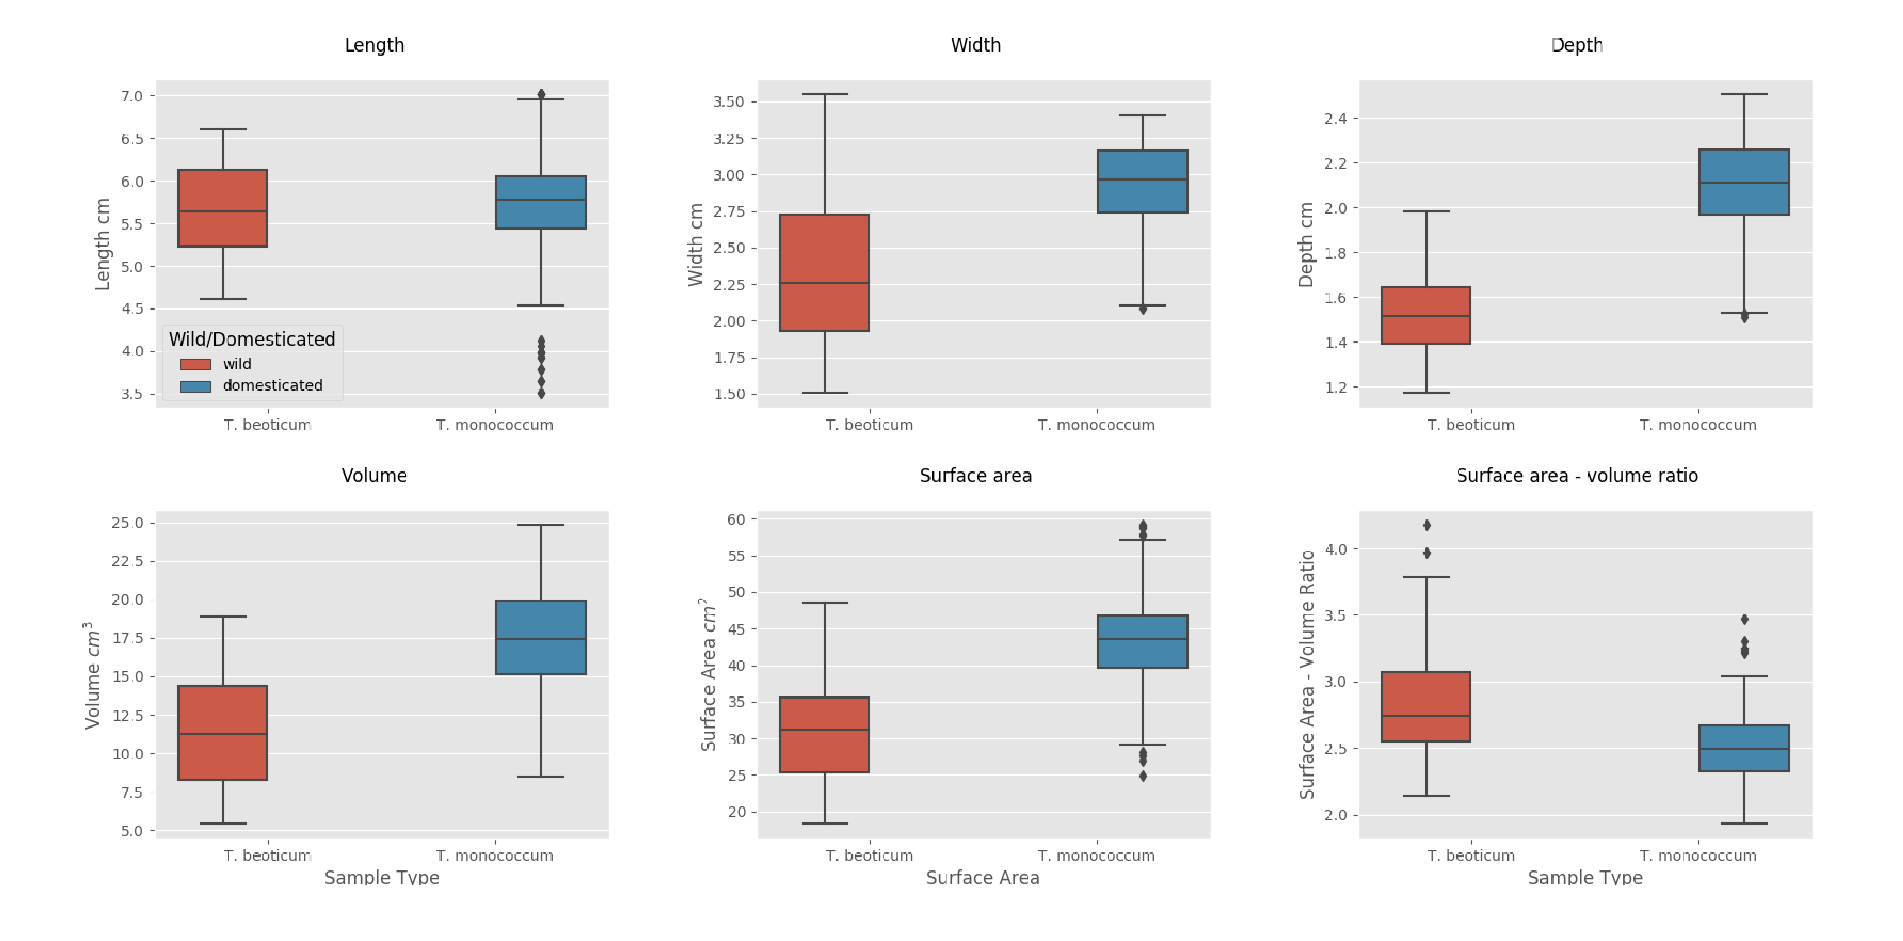
\includegraphics[width=.9\linewidth]{./einkorn.png}
\caption{\label{fig:org62f1159}
einkorn table}
\end{figure}


\subsection{emmer}
\label{sec:org7266207}
\begin{figure}[htbp]
\centering
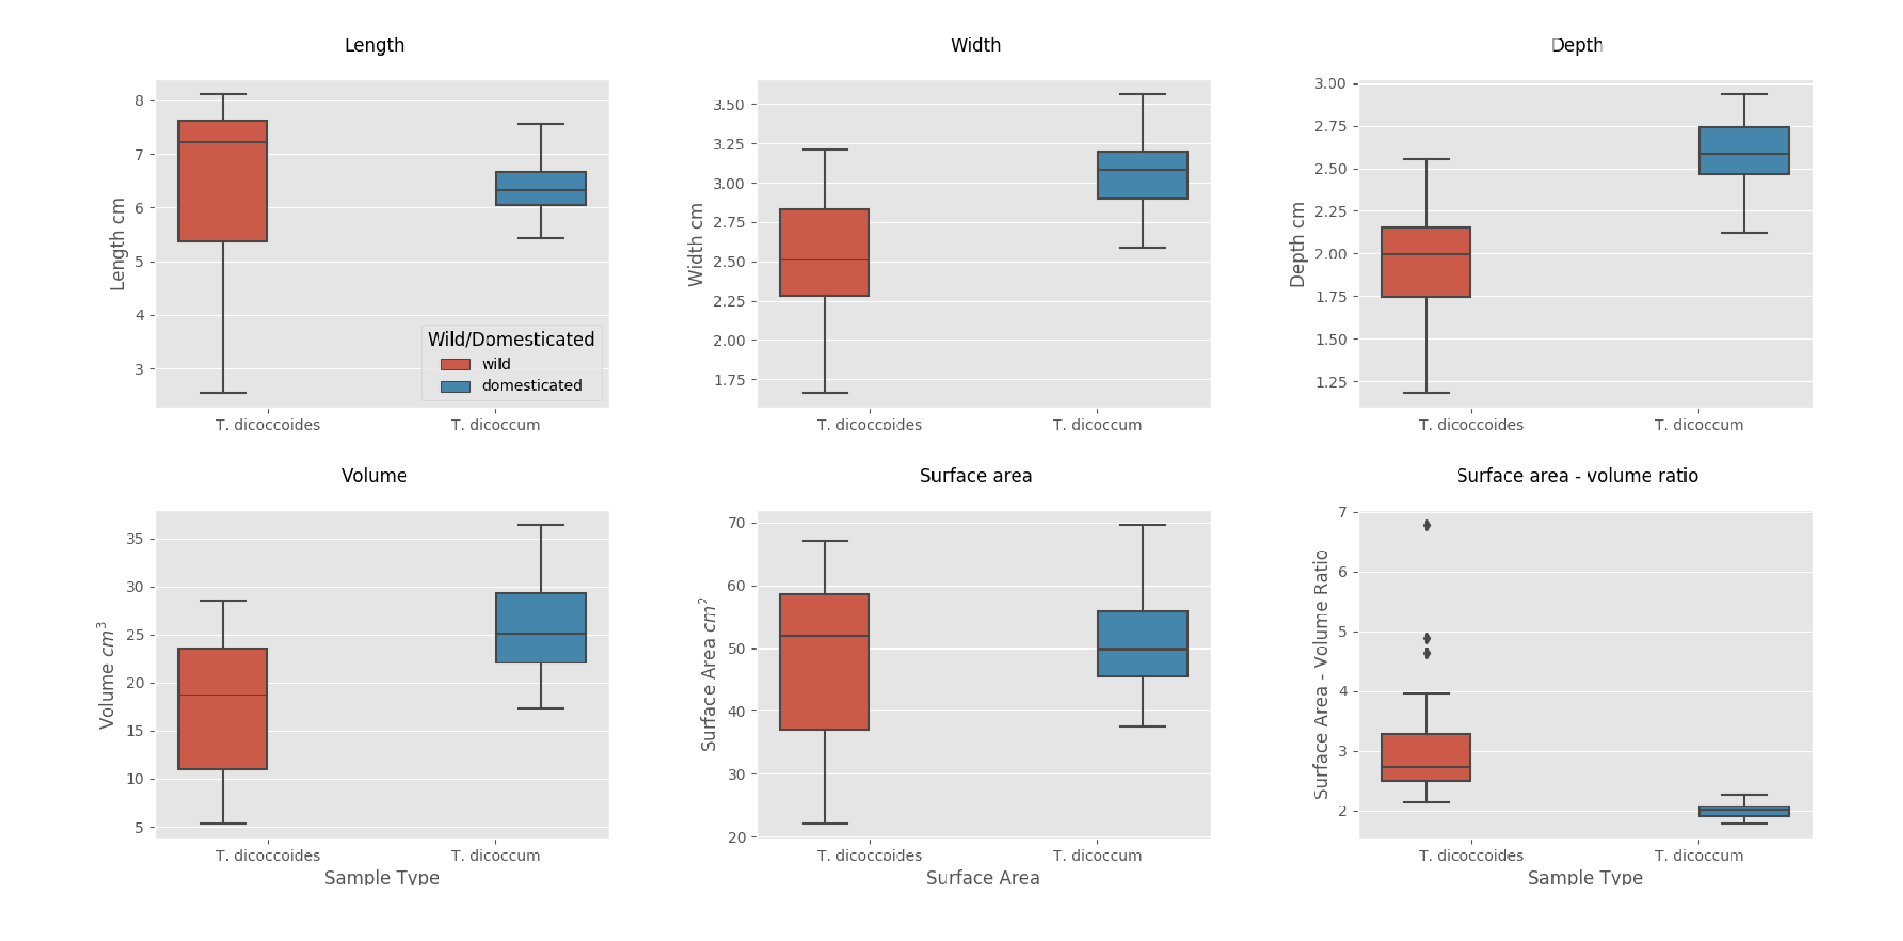
\includegraphics[width=.9\linewidth]{./emmer.png}
\caption{\label{fig:org60d0038}
emmer table}
\end{figure}

\clearpage


\subsection{Barley}
\label{sec:orgf491518}
\begin{figure}[htbp]
\centering
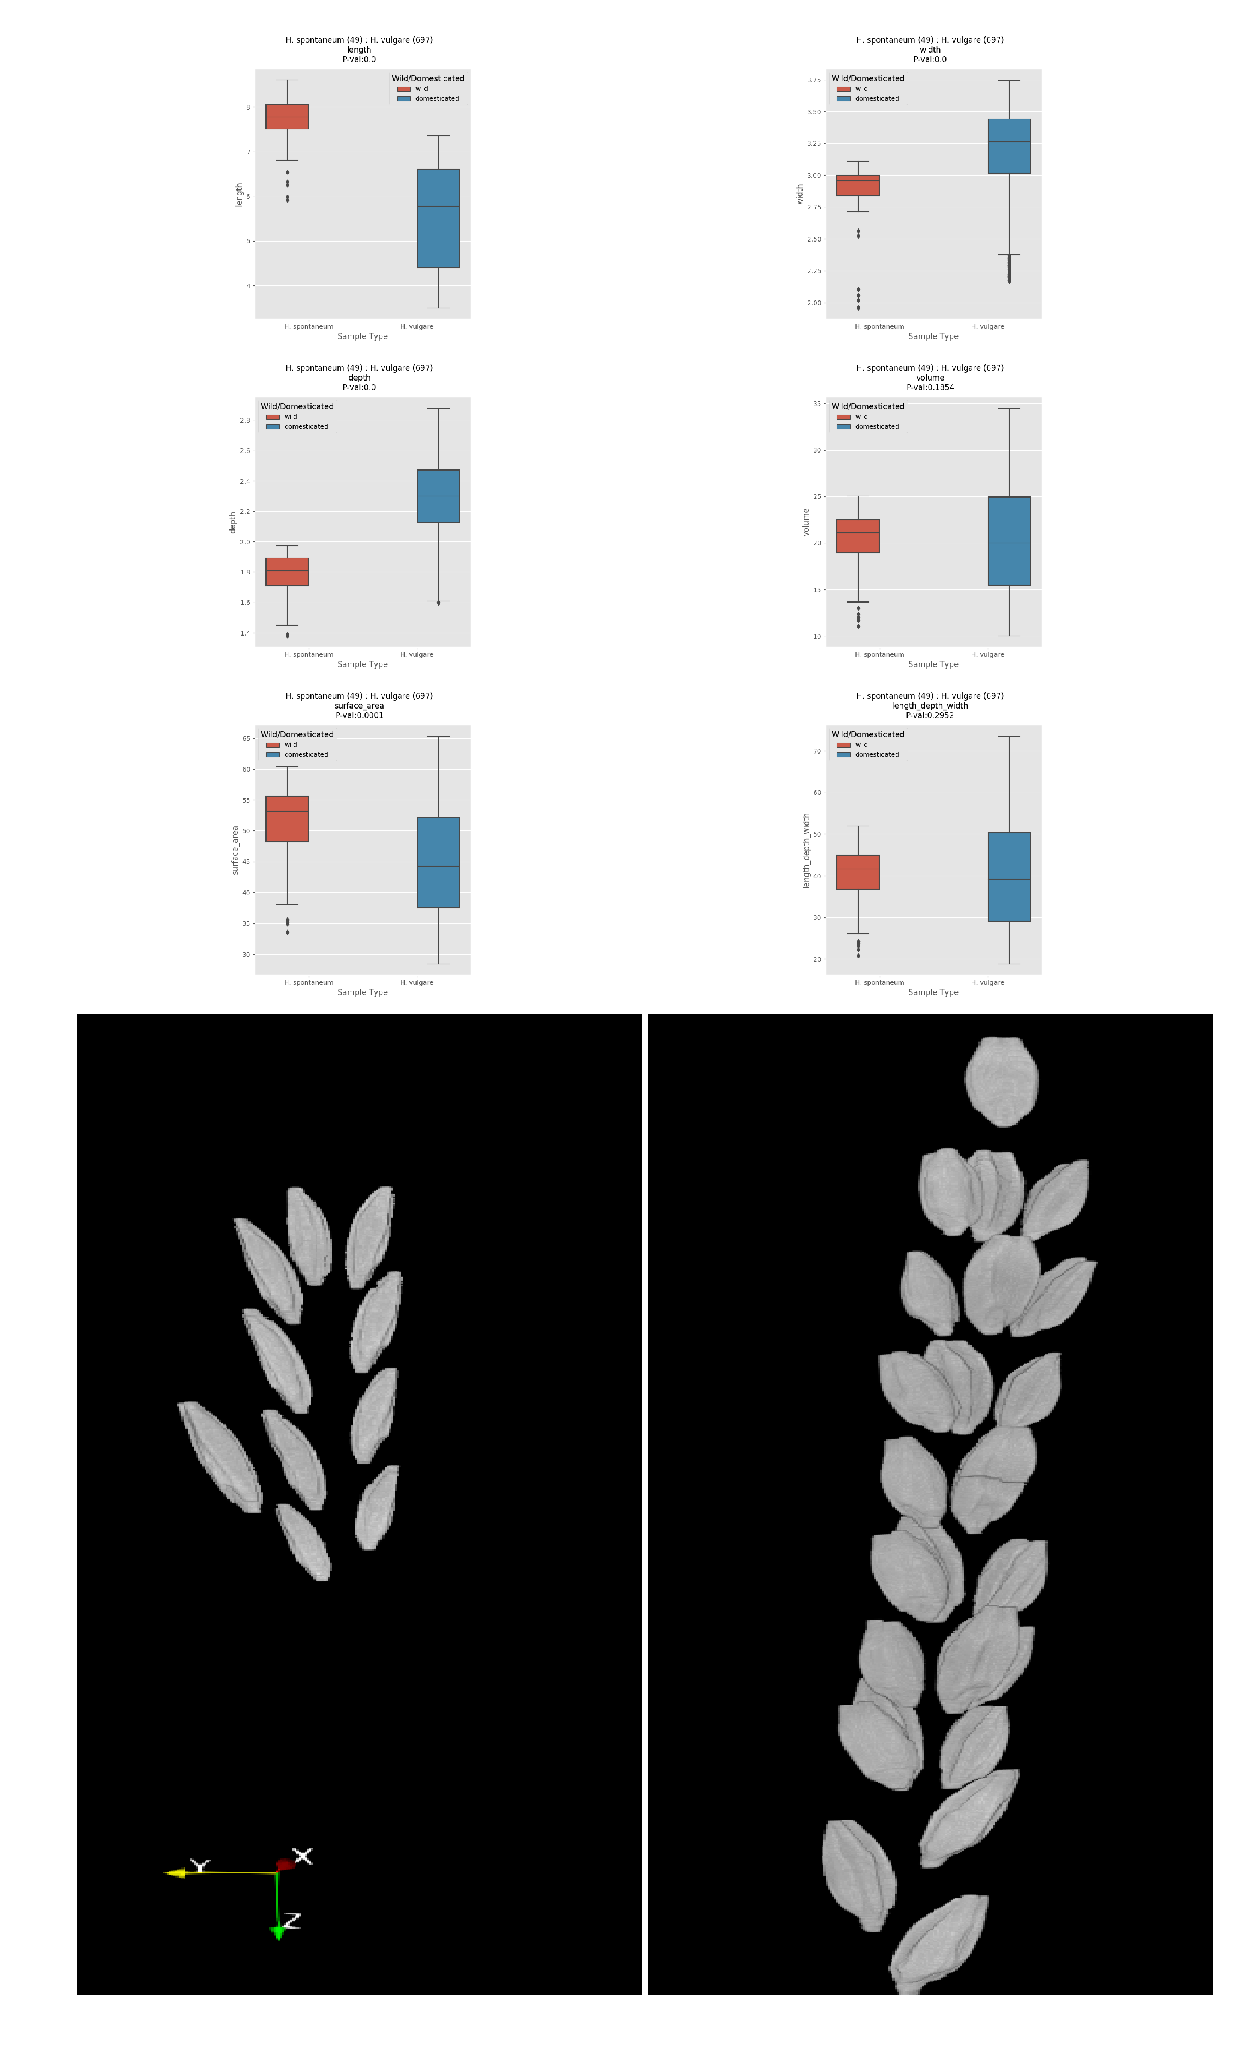
\includegraphics[width=.9\linewidth]{./barley.png}
\caption{\label{fig:org6fcf241}
barley table}
\end{figure}


\subsection{Domesticated 2N, 4N}
\label{sec:org55f6d89}
\begin{figure}[htbp]
\centering
\includegraphics[width=.9\linewidth]{./dom.png}
\caption{\label{fig:org778d7cd}
domesticated 2N, 4N table}
\end{figure}

\clearpage
\subsection{Wild 2N, 4N}
\label{sec:org6a1967a}
\begin{figure}[htbp]
\centering
\includegraphics[width=.9\linewidth]{./wild.png}
\caption{\label{fig:org11bf147}
wild 2N, 4N  table}
\end{figure}

\clearpage

\bibliography{library}
\bibliographystyle{unsrt}
\end{document}